\section{Background Estimation}
\label{sec:background_estimation}
In order to estimate the expected background in the Low Energy and Mid Energy samples, a data based technique was used which minimizes the effect of any systematic uncertainties on the background estimate. For a detector operated uniformly over a long period of time, different right ascensions at the same declination will all correspond to the same set of directions in detector coordinates.  This means that the expected background in a cone around the galactic center can be estimated by counting all events in the same declination band as the cone.  In order to avoid contaminating the background estimate with a potential signal excess from the search cone, only events with $\theta_\textrm{GC}>80^\circ$ are included in the background estimate.  The background estimate ``Away From Source" (AFS) region and search cone are shown for a 25$^\circ$ degree cone around the Galactic Center in \cref{fig:afs_regions_skymap}. 
 

\begin{figure} 
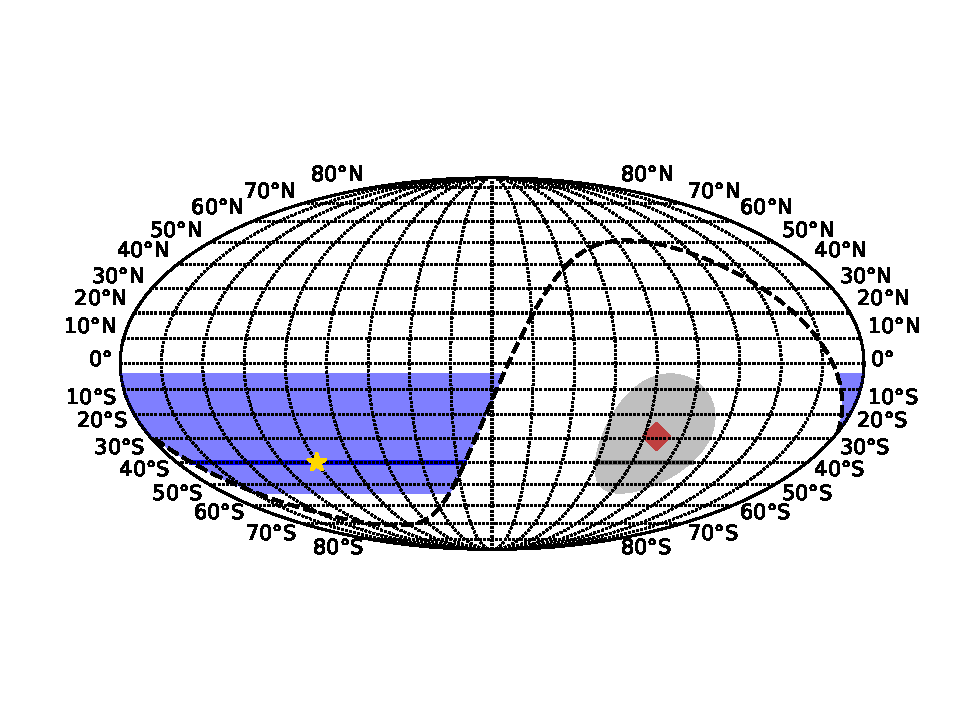
\includegraphics[width=0.45\textwidth]{figures/AFS_witharcs.pdf}
\caption{``Away From Source" (AFS) region shown in blue, and search cone shown in gray for a search cone of 25$^\circ$ half-opening angle around the galactic center.  The red diamond it at the location of the galactic center.  The dotted black line represents the 80$^\circ$ cone outside of which the AFS region is defined.  For an event at the location of the yellow start, the weight for background estimation is the ratio of the gray arc to the blue arc.}
\label{fig:afs_regions_skymap}
\end{figure}

Since at the same declination the AFS region and search cone span different amounts of right ascension, events found in the AFS region must be weighted according to their declination in order to find the correct background estimate for the search cone.  The weight of each event in the AFS region is equal to the ratio of right ascensions spanned by the search cone to right ascensions spanned by the AFS region at that declination, which is visualized in \cref{fig:afs_regions_skymap,fig:afs_weight_calc_cones} .  
\begin{figure*} 
       \centering
	\subfigure[]{
 		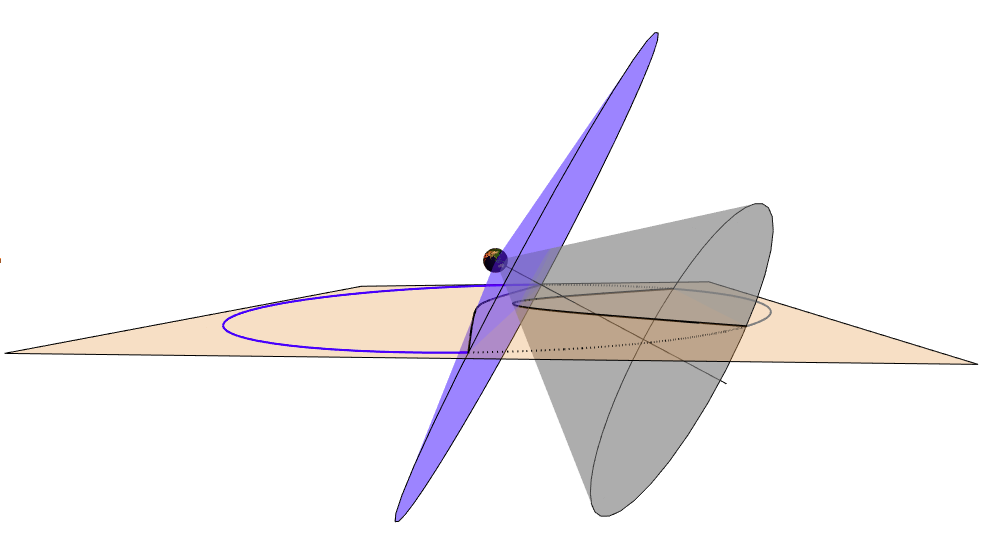
\includegraphics[width=0.45\textwidth]{figures/AFS_weght_calc_cones.png}
 		\label{fig:afs_weight_calc_cones}
}
	\subfigure[]{
 		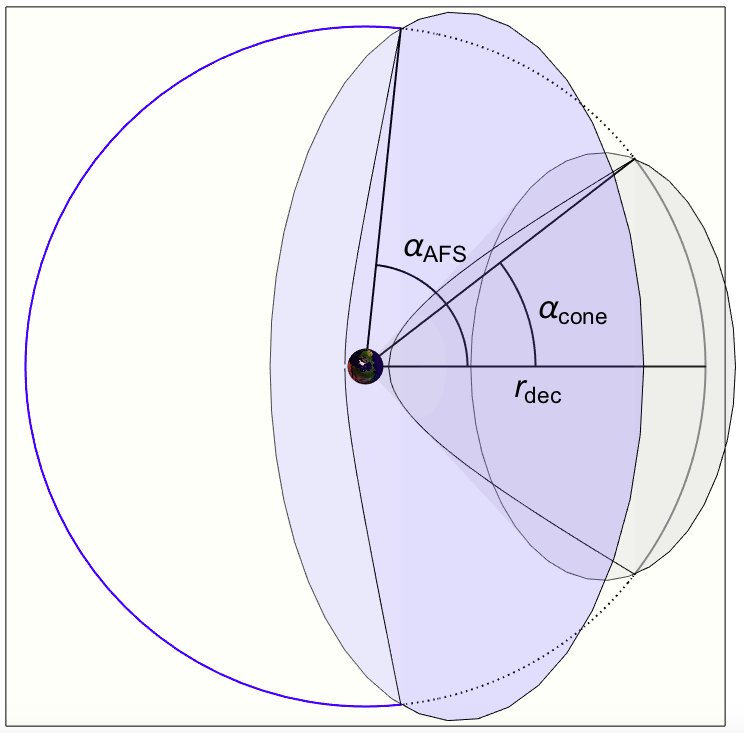
\includegraphics[width=0.45\textwidth]{figures/AFS_weght_calc_cones_rotated.png}
 		\label{fig:afs_weight_calc_cones_rotated}
}
\caption{Visualization of the event weighting for background estimation.  An event found in the AFS region at the declination respresented by the plane is weighted by the ratio of the gray arc to the blue arc.  Figure \ref{fig:afs_weight_calc_cones_rotated} shows Figure \ref{fig:afs_weight_calc_cones} as seen from directly above.  The Mathematica code used to create these images can be found in \cref{app:mathematica}} 
\end{figure*}
This weight can be written in terms of the variables in Figure \ref{fig:afs_weight_calc_cones_rotated} as $w=\frac{\alpha_\textrm{cone}}{\pi-\alpha_\textrm{AFS}}$.  To compute $\alpha_\textrm{cone}$ and $\alpha_\textrm{AFS}$, the points must be found where a cone of half opening angle $\theta$ centered on the direction to the galactic center, a plane at declination $\phi_\textrm{dec}$, and the unit sphere intersect.  (The directions are without loss of generality assumed to be unit vectors, thus the inclusion of the unit sphere requirement).  In \cref{fig:afs_weight_calc_cones}, for the AFS region (GC search cone), these points are at the intersection of the blue (gray) cone, pink plane, and the circle drawn on the plane.  The circle in \cref{fig:afs_weight_calc_cones_rotated} is the intersection of the plane and the unit sphere, and so $r_\textrm{dec}=\cos \phi_\textrm{dec}$.  Defining the x-axis as pointing toward the right ascension of the galactic center at declination 0, the z-axis as extending from the poles of the earth so that +$\hat{z}$ correspondes with a declination of 90$^\circ$ and -$\hat{z}$ with a declination of -90$^\circ$, and the y-axis accordingly to keep the coordinate system right handed, we can write the position of the two intersection points as:
\begin{equation}
\hat{v}_\pm=(x',\pm y',z')
\end{equation} 
and the Galactic Center direction as:
\begin{equation}
\hat{v}_\textrm{GC}=(\cos (-29^\circ),0,\sin (-29^\circ))
\end{equation}
Since $\hat{v}_\pm$ are on the plane at declination $\phi_\textrm{dec}$ we have:
\begin{equation}
z'=\sin \phi_\textrm{dec}
\end{equation}
Additionally, since $\hat{v}_\pm$ are on the cone of half opening angle $\theta$ around the Galactic Center we have 
\begin{eqnarray}
\label{eq:cone_condition_1}
\frac{|\hat{v}_\pm-(\hat{v}_\pm \cdot \hat{v}_\textrm{GC})\hat{v}_\textrm{gc}|}{|(\hat{v}_\pm \cdot \hat{v}_\textrm{GC})\hat{v}_\textrm{GC}|}=\tan \theta
\\
\hat{v}_\pm \cdot \hat{v}_\textrm{GC}>0
\label{eq:cone_condition_2}
\end{eqnarray}

Solving Equation \ref{eq:cone_condition_1} under the condition of Equation \ref{eq:cone_condition_2}, we have:
\begin{eqnarray}
\frac{\sqrt{(\hat{v}_\pm-(\hat{v}_\pm \cdot \hat{v}_\textrm{GC})\hat{v}_\textrm{GC})\cdot(\hat{v}_\pm-(\hat{v}_\pm \cdot \hat{v}_\textrm{GC})\hat{v}_\textrm{GC})}}{\sqrt{((\hat{v}_\pm \cdot \hat{v}_\textrm{GC})\hat{v}_\textrm{GC})\cdot((\hat{v}_\pm \cdot \hat{v}_\textrm{GC})\hat{v}_\textrm{GC})}}=\tan \theta\\
\frac{\sqrt{\hat{v}_\pm\cdot\hat{v}_\pm+(\hat{v}_\textrm{GC} \cdot \hat{v}_\textrm{GC}-2)(\hat{v}_\pm \cdot \hat{v}_\textrm{GC})^2 }}{\sqrt{(\hat{v}_\pm \cdot \hat{v}_\textrm{GC})^2\hat{v}_\textrm{GC} \cdot \hat{v}_\textrm{GC}}}=\tan \theta\\
\frac{\sqrt{1-(\hat{v}_\pm \cdot \hat{v}_\textrm{GC})^2}}{\hat{v}_\pm \cdot \hat{v}_\textrm{GC}}=\tan \theta \\
1-(\hat{v}_\pm \cdot \hat{v}_\textrm{GC})^2=\tan^2 \theta (\hat{v}_\pm \cdot \hat{v}_\textrm{GC})^2\\
\hat{v}_\pm \cdot \hat{v}_\textrm{GC}=\sqrt{\frac{1}{1+\tan^2\theta}}\\
x'\cos (-29^\circ)+\sin \phi_{dec} \sin (-29^\circ)=\sqrt{\frac{1}{1+\tan^2\theta}}\\
x'=\frac{-\sin \phi_{dec} \sin (-29^\circ)+\sqrt{\frac{1}{1+\tan^2\theta}}}{\cos (-29^\circ)}
\end{eqnarray}
where we have used the fact that $(\hat{v}_\textrm{GC} \cdot \hat{v}_\textrm{GC} )=(\hat{v}_\pm \cdot \hat{v}_\pm)=1$.
The angle $\alpha$ is then found as 
\begin{equation}
\cos \alpha=\frac{x'}{r_\textrm{dec}}=\frac{-\sin \phi_{dec} \sin (-29^\circ)+\sqrt{\frac{1}{1+\tan^2\theta}}}{\cos (-29^\circ) \cos \phi_\textrm{dec}}
\end{equation}
The weight for an event in the AFS region at declination $\phi_\textrm{dec}$ can thus be found as 
\begin{eqnarray}
&w(\phi_\textrm{dec})=\frac{\alpha_\textrm{cone}}{\pi-\alpha_\textrm{AFS}} \\
&\cos \alpha_\textrm{cone}=\frac{-\sin \phi_{dec} \sin (-29^\circ)+\sqrt{\frac{1}{1+\tan^2\theta_\textrm{cone}}}}{\cos (-29^\circ) \cos \phi_\textrm{dec}} \\
&\cos \alpha_\textrm{AFS}=\frac{-\sin \phi_{dec} \sin (-29^\circ)+\sqrt{\frac{1}{1+\tan^2\theta_\textrm{AFS}}}}{\cos (-29^\circ) \cos \phi_\textrm{dec}} 
\label{eq:weight}
\end{eqnarray}
The background estimate and uncertainty on the estimate are then
\begin{eqnarray}
B_\textrm{est}=\sum \limits_i w(\phi_{\textrm{dec},i})
\\
\sigma B_\textrm{est}=\sqrt{\sum \limits_i w^2(\phi_{\textrm{dec},i})}.
\label{eq:bckg_est}
\end{eqnarray}

A similar technique could be applied to the search around the sun, however the declination of the sun changes with time, and so them math becomes more complicated.  Instead, a slightly different approach was taken.  The search cone for the solar search is a 5$^\circ$ cone around the sun, and everything outside of this cone is taken as the AFS region.  For an event in the AFS region, the correct weight to use for background estimation is then the ratio of time that the horizontal coordinate direction of the event is within the 5$^\circ$ cone around the sun to the time it is outside the cone.  These weights are calculated as follows.  Direction in horizontal coordinates are divided into a grid of 1000 bin in azimuth by 600 bins in cosine zenith.  The weight for events in each bin is then computed by stepping through a year in steps of 1 second and counting up the amount of time each bin is within 5$^\circ$ of the sun.  The fraction of time spent within $5^\circ$ of the sun as a function of cosine zenith and azimuth is shown in \cref{fig:pos_sun}

\begin{figure}
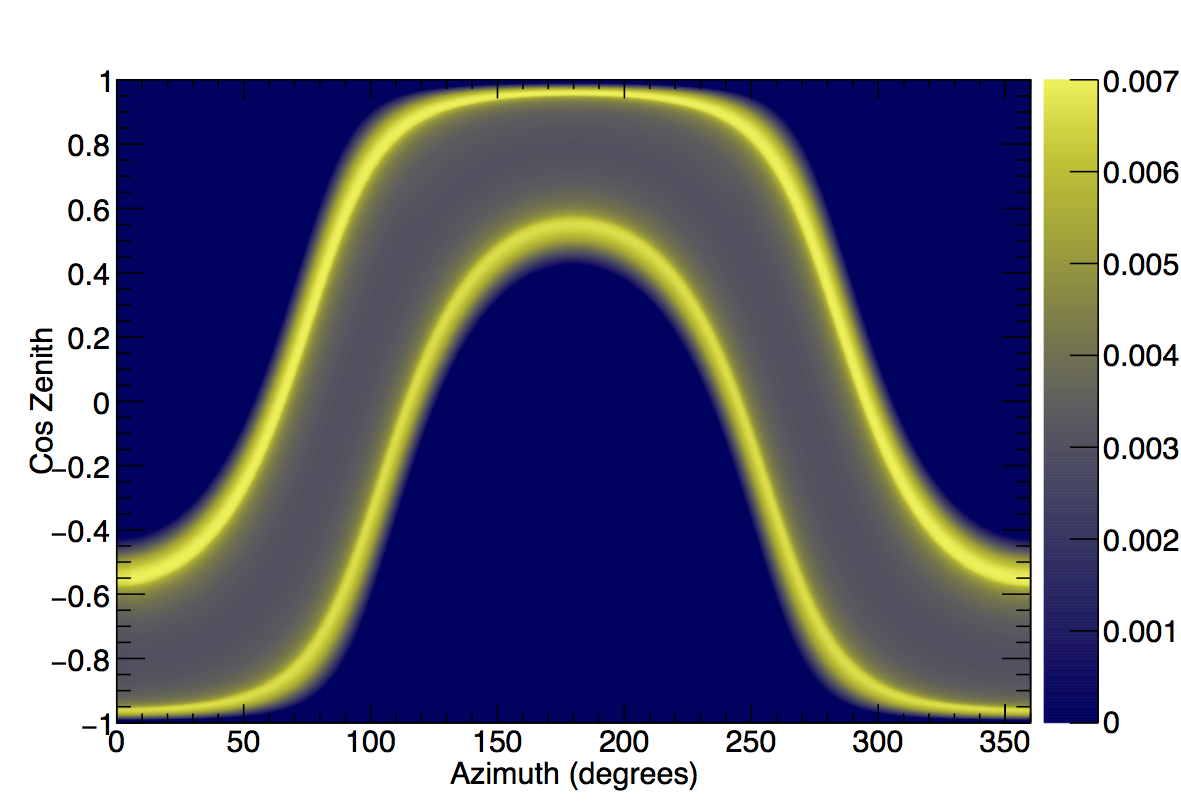
\includegraphics[width=0.45\textwidth]{figures/pos_sun.png}
\caption{The fraction of time spent with $5^\circ$ of the sun, as a function of cosine zenith and azimuth.  }
\label{fig:pos_sun}
\end{figure}   

In both the application to the galactic center and to the sun it is implicitly assumed that the detector has been run uniformly in time.  This assumption could introduce error in the background estimates if instead the detector has run much more at certain times of the day or year than at others.  Therefore 500 years of atmospheric neutrino MC was used to test the validity of the AFS method.  The time of each MC event was chosen from the times of real data events.  The AFS method was the applied to the MC.  The background estimate made by the AFS method applied to the MC was compared to the number of events found in the search cone in the MC.  If these numbers were found to be very different, it would indicate non-uniformity of the time when the detector has been run is leading to a bias in the AFS background estimate.  As can be seen in \cref{fig:AFS_verification}, the difference is both statistically consistent with 0, and much smaller than the uncertainty in the AFS background estimates when applied to real data.  Therefore, any potential bias in the AFS method introduced by non-uniform running of the detector can be ignored.  


\begin{figure*}
 	\centering
	\subfigure[Low Energy]{
  	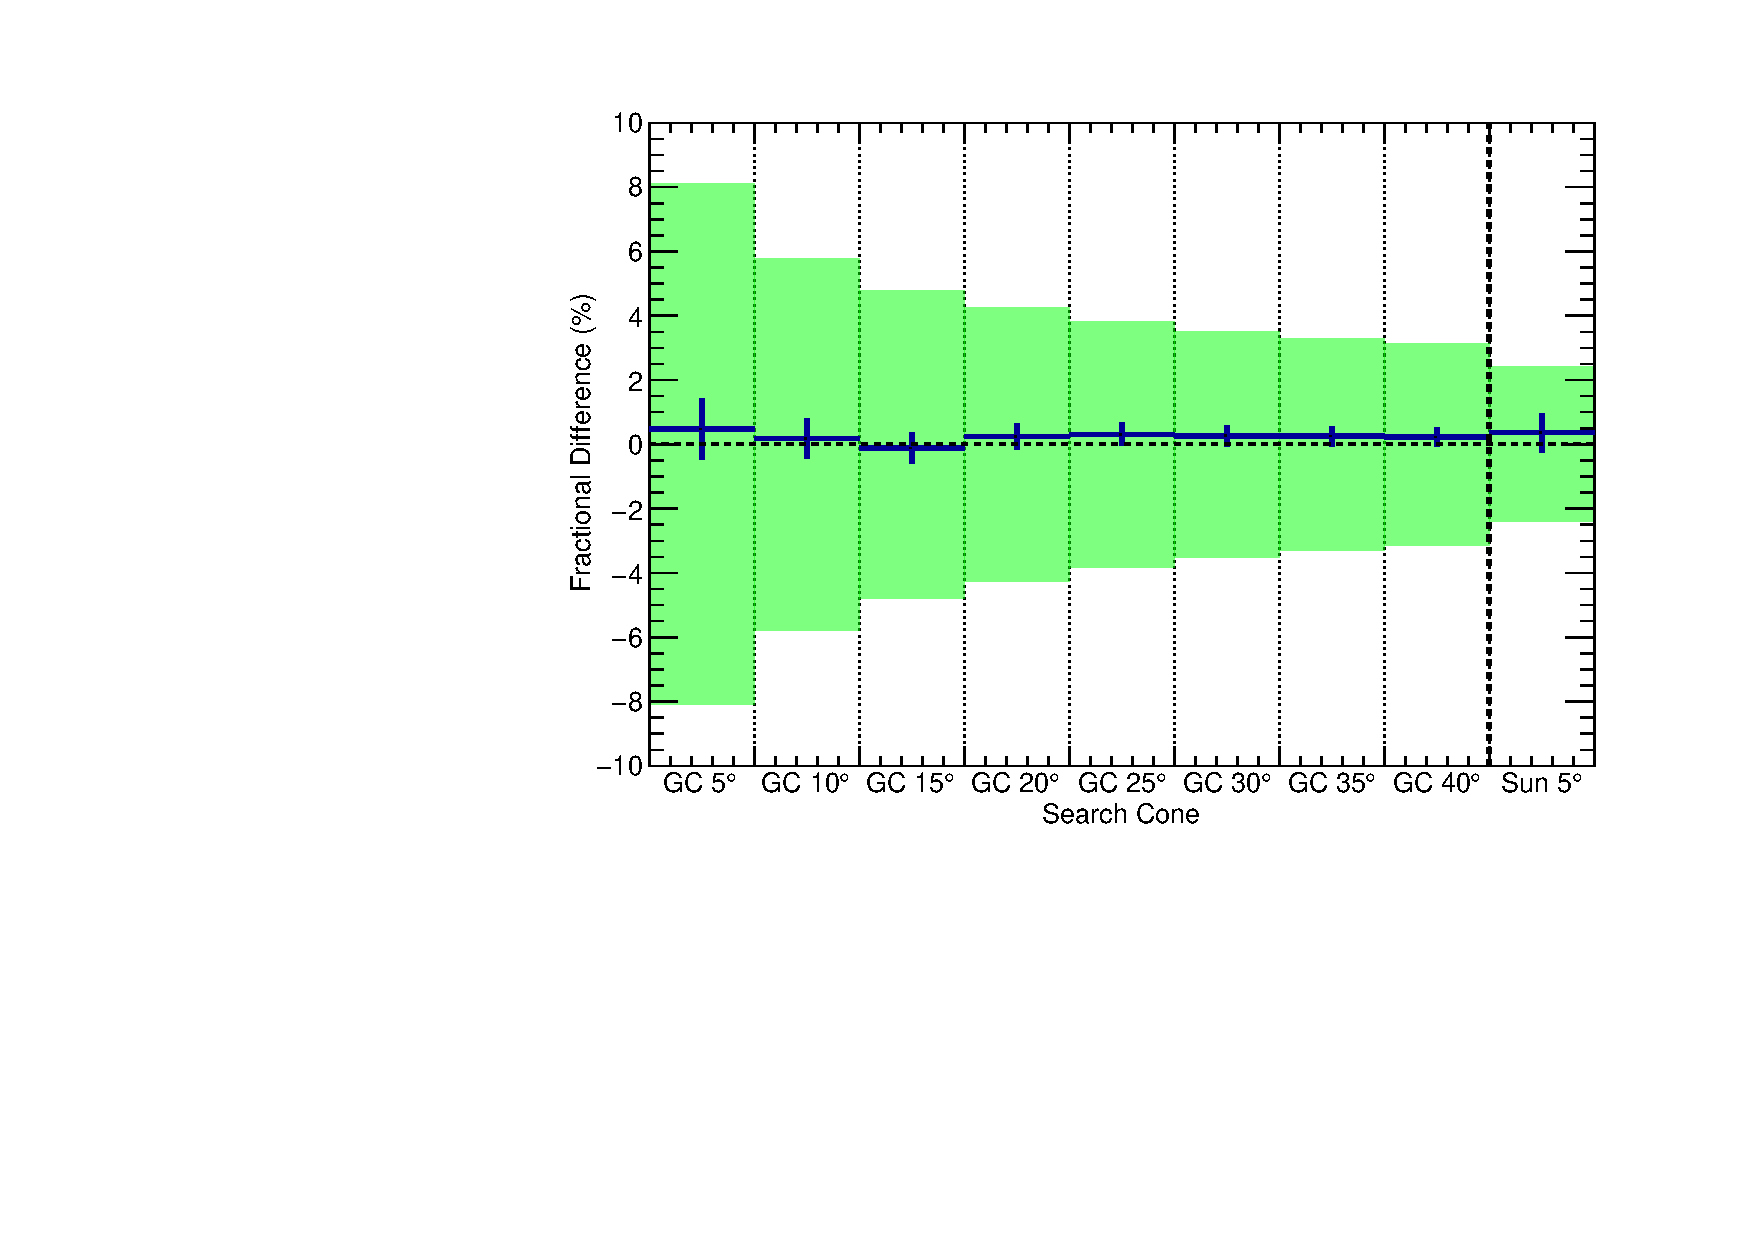
\includegraphics[width=0.45\textwidth]{figures/AFS_verification_SubGeV.pdf}
	}
	\subfigure[Mid Energy]{
 	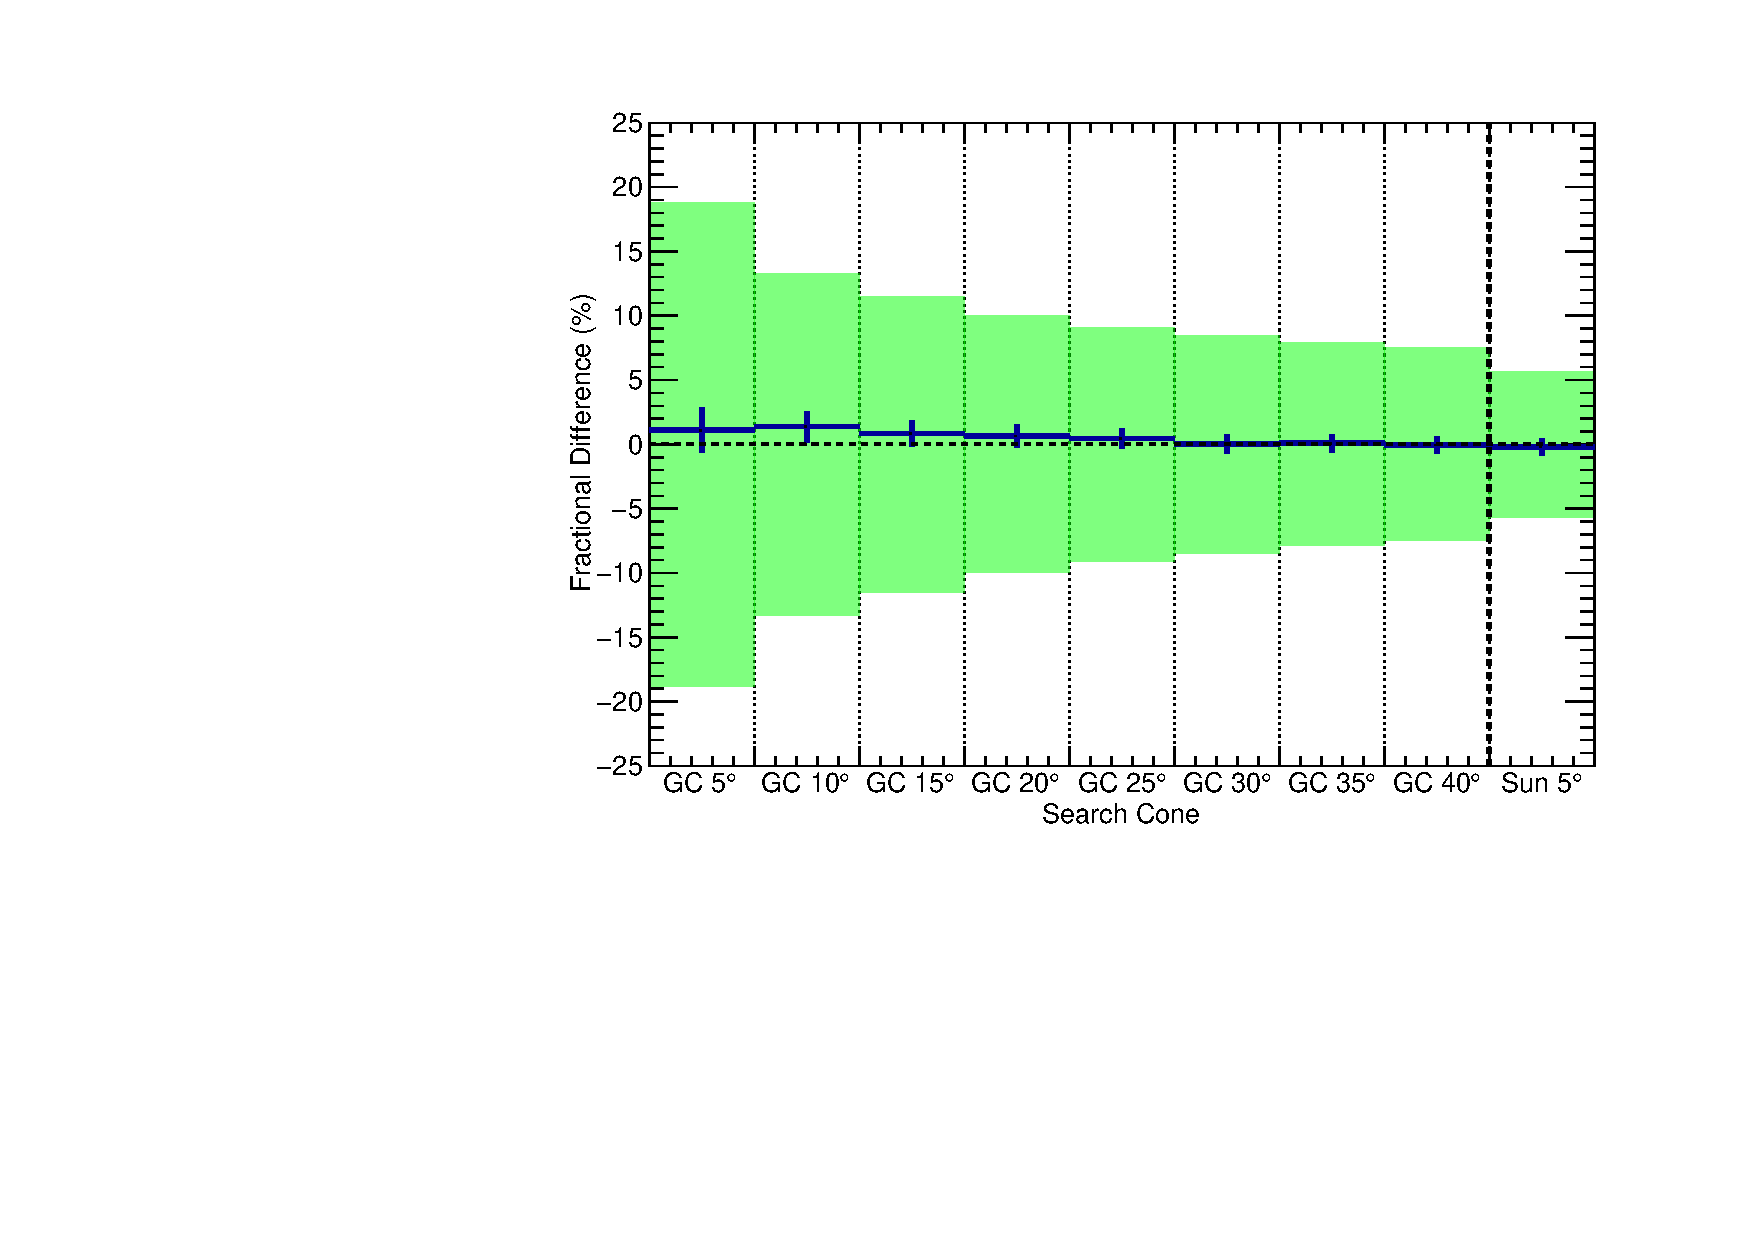
\includegraphics[width=0.45\textwidth]{figures/AFS_verification_MidEnergy.pdf}
	}
	\caption{Verification of AFS method.  The blue histogram shows the fractional difference between the AFS background estimate when applied to MC and the actual number of events in the search cone in MC.  The green shows the AFS background estimate uncertainty when applied to data. }
	\label{fig:AFS_verification} 
\end{figure*}  

For the High Energy event sample, there would be too few events in the AFS region for the above technique to work well.  Instead, the MC estimate for the expected number of atmospheric neutrino events in the search cone was taken as the background estimate.  The MC was livetime normalized and oscillated according to 3-flavor oscillations with oscillation parameters $\Delta M_{23}^2=2.5 \times 10^{-3}$ GeV$^2$, $\Delta M_{12}^2=7.65 \times 10^{-5}$ GeV$^2$, $\sin^2 \theta_{23}=0.5875, \sin^2 \theta_{13}=0.0219, \sin^2 \theta_12=0.309, \delta_{cp}=4.19$.   The systematic uncertainty on this estimate if found by summing in quadrature the effect of and 1-$\sigma$ shift of all 75 official SK-IV systematics.  The uncertainty of oscillation parameters were also included as systematics. Of these only 18 cause more than a 1\% shift in our background estimate at 1-$\sigma$.  The uncertainties which cause more than a 5\% shift at 1-$\sigma$ are shown in Table \ref{tab:systematics}.   As seen in Table \ref{tab:systematics}, the systematic uncertainty of the Higher Energy sample is dominated by the systematic uncertainty of the neutron tagging cut.  This uncertainty accounts for the uncertainty in the efficiency of our neutron tagging algorithm, as well as the uncertainty in the production and transport of neutrons in the detector.  It was estimated by a Data-MC comparison of the fraction of events passing the first three selection cuts which also had zero tagged neutrons as a function of visible energy.  Above about 10 GeV of visible energy, there are very low statistics for the data, and so a Data-MC comparison is difficult to make.  Therefor, above 3 GeV both the data and MC were fitted to logarithmic functions $A+B\log \frac{\textrm{E}_\textrm{vis}}{\textrm{GeV}}$, as shown in Figure \ref{fig:ntag_syst_err_0frac}.  The systematic uncetainty was then taken as the difference between the Data fit and the MC fit in the region above 7.6 GeV of visible energy.  The total uncertainty for the High Energy event sample is 29.8\%.    

The background estimate results for the 8 cone sizes around the galactic center and the $5^\circ$ cone around the Sun are shown in \cref{tab:backg_est}.  The background estimates for the low and mid energy regions are compared to MC background estimates in \cref{fig:bckg_comparison}.  The systematic uncertainties on the MC background estimates for the low and mid energy samples were computed in the same way as for the high energy sample, resulting is uncertainties of 18.4\% and 17.7\% respectively.  As can be seen in \cref{fig:bckg_comparison}, the two background estimation techniques agree with one another to within systematic uncertainties, and the systematic uncertainties on the AFS technique are much smaller than those on the MC based estimate. 


\begin{table}[h]
\begin{tabular}{lc}
\hline \hline
Systematic& 1-$\sigma$ shift \\
\hline
Neutron Tagging Cut & 23\%\\
Normalization (Flux, Data reduction, FV) & 11\% \\
Energy Calibration & 6\% \\
Garczyk and Socyzk 1$\pi$ axial coupling & 5\% \\
\hline
\end{tabular}
\caption{Largest systematic uncertainty contributions for High Energy sample.}
\label{tab:systematics}
\end{table}     


\begin{figure*}
	\centering
	\subfigure[]{
		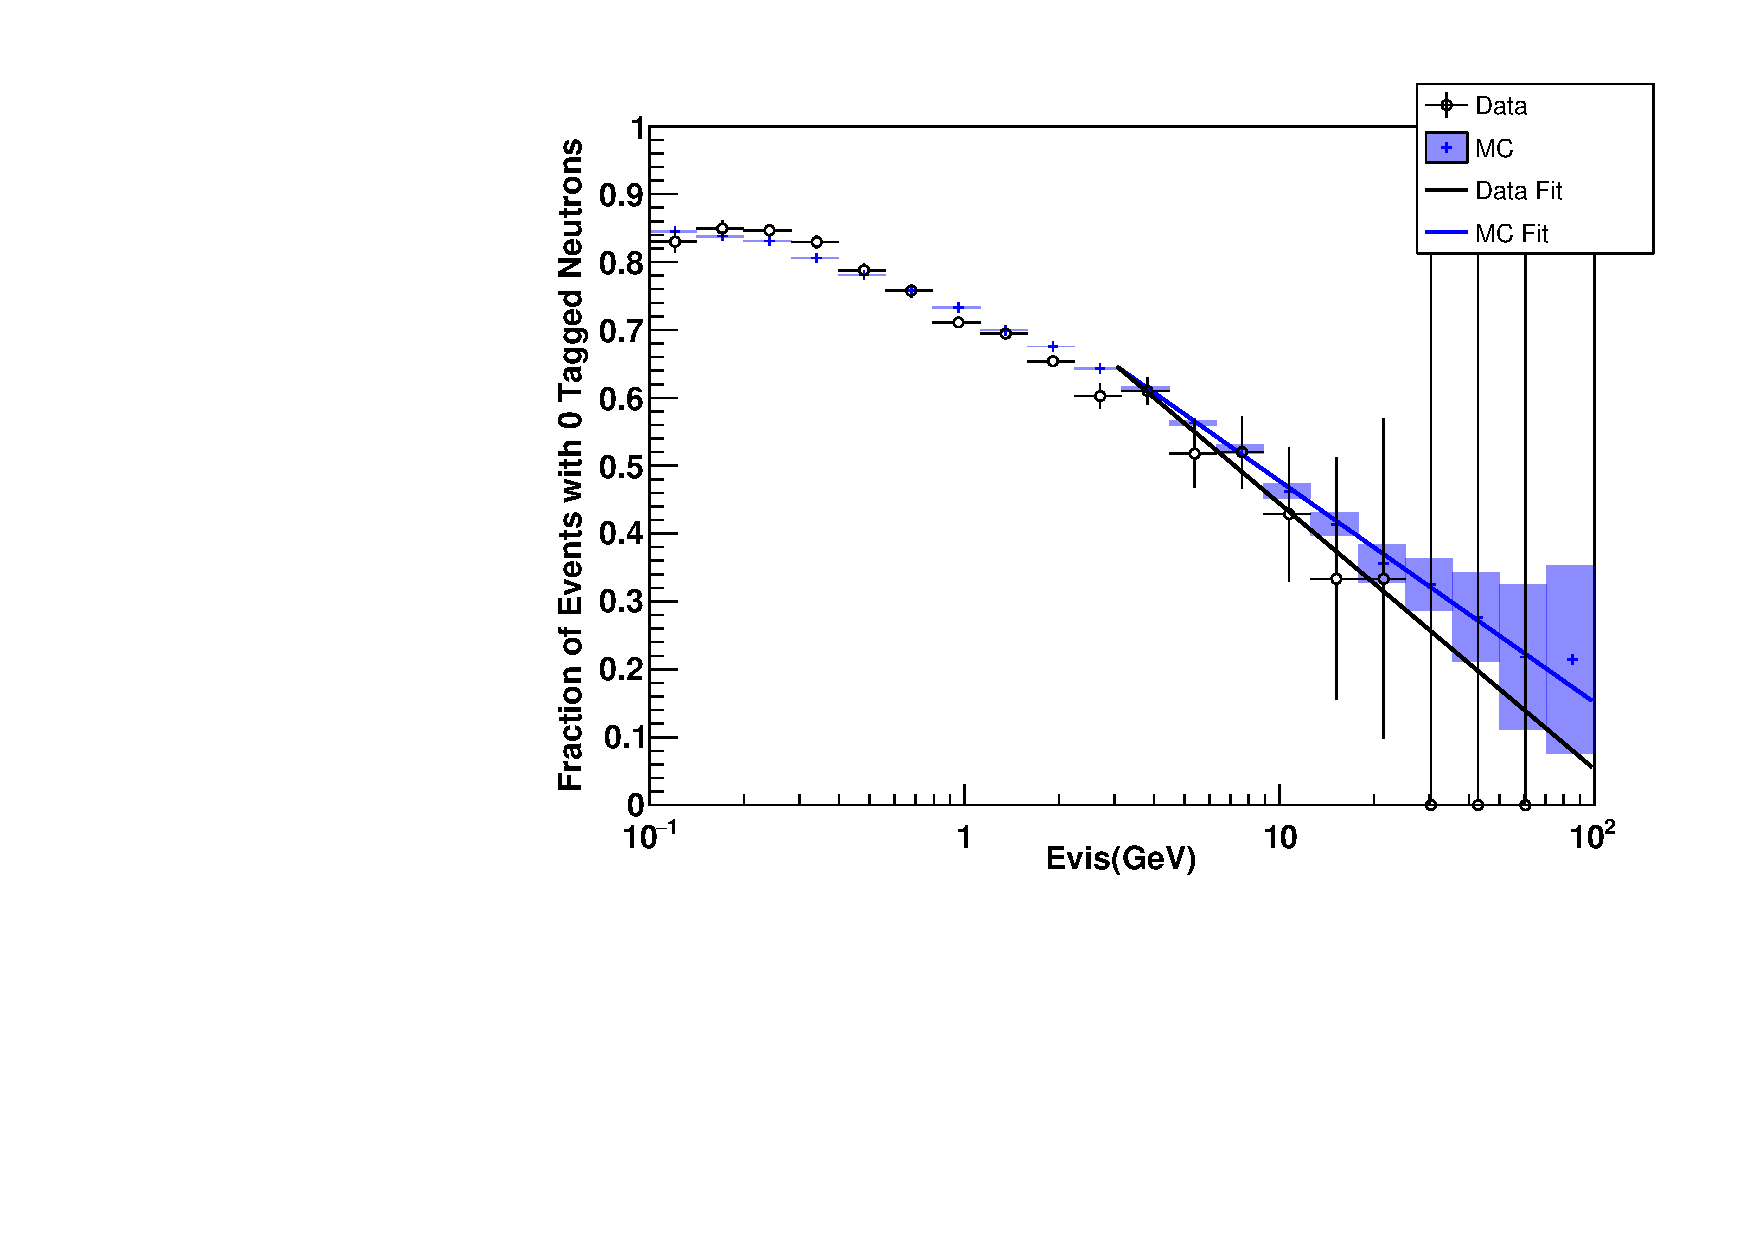
\includegraphics[width=0.45\textwidth]{figures/ntag_syst_err_0frac.pdf}
		\label{fig:ntag_syst_err_0frac}
	}
	\subfigure[]{
		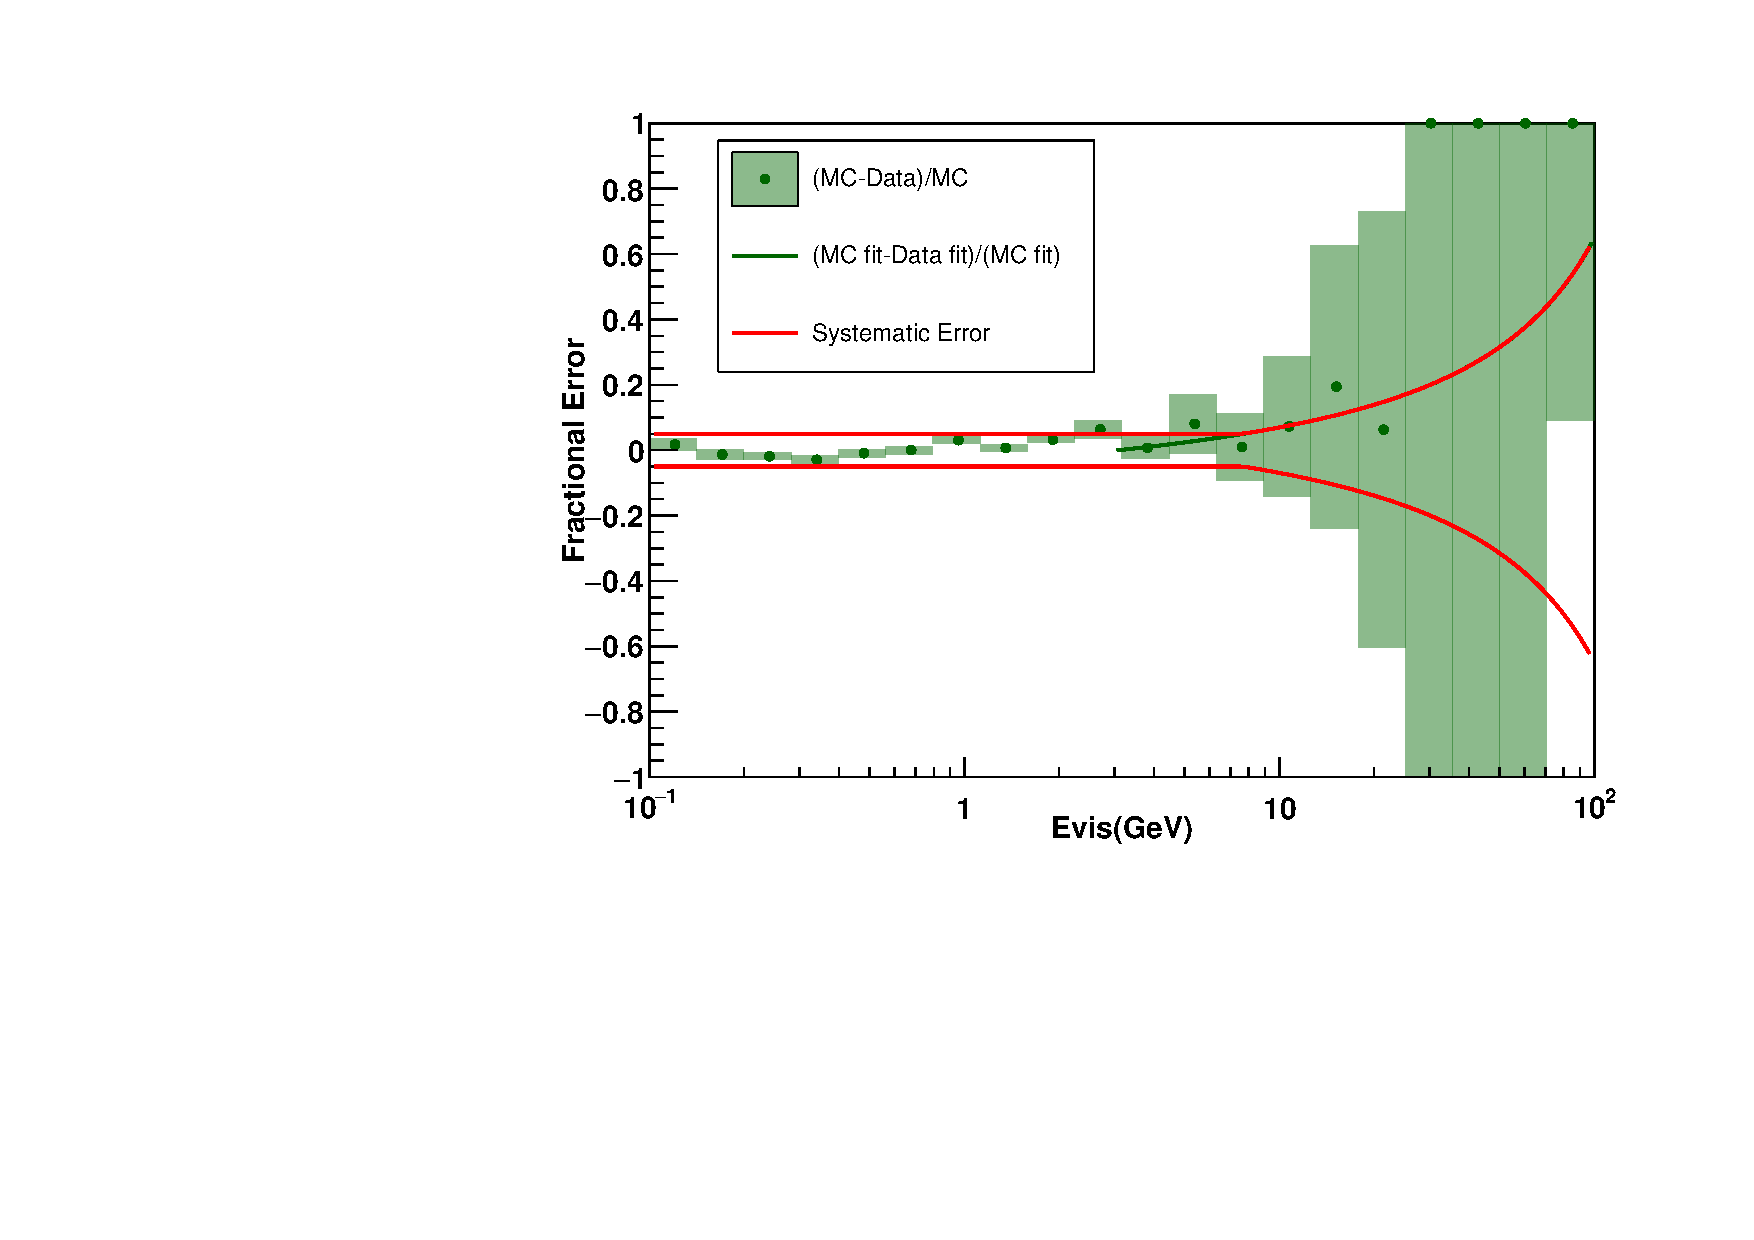
\includegraphics[width=0.45\textwidth]{figures/ntag_syst_err_final.pdf}
		\label{fig:ntag_syst_err_final}
	}
	\caption{Neutron tagging cut systematic error estimation.  \ref{fig:ntag_syst_err_0frac} shows the fractional number of events passing the neutron tagging cut after passing all previous cuts for both Data and MC, along with logarithmic fits. The filled rectangles around the MC show statistical uncertainty in the MC. \ref{fig:ntag_syst_err_final} shows the resulting systematic uncertainty, set to 5\% below 7.6 GeV, and the difference in the two fits from \ref{fig:ntag_syst_err_0frac} above 7.6 GeV.}
\label{fig:ntag_syst}
\end{figure*}


\begin{table}[h]
\resizebox{\textwidth}{!}{
\begin{tabular}{lccc}
\hline\hline
&Low Energy&Mid Energy&High Energy\\
\hline
GC 5$^\circ$ cone & $8.6 \pm 0.7$ & $1.6 \pm 0.3$ & $0.011 \pm 0.003$\\

GC 10$^\circ$ cone& $32.9 \pm 1.9$ & $6.3 \pm 0.84$ & $0.041 \pm 0.012$ \\

GC 15$^\circ$ cone& $74.4 \pm 3.6$ & $13.9 \pm 1.6$ & $0.096 \pm 0.029$\\

GC 20$^\circ$ cone& $129.9 \pm 5.5$ & $23.9 \pm 2.4$ & $0.17 \pm 0.05$\\

GC 25$^\circ$ cone& $201.4 \pm 7.7$ & $36.4 \pm 3.3$ & $0.26 \pm 0.08$\\

GC 30$^\circ$ cone& $290.3 \pm 10.2$ & $50.6 \pm 4.3$ & $0.37 \pm 0.11$\\
 
GC 35$^\circ$ cone& $394.1 \pm 13.0$ & $69.7 \pm 5.5$ & $0.49 \pm 0.15$\\

GC 40$^\circ$ cone& $511.2 \pm 16.0$ & $92.1 \pm 6.9$ & $0.63 \pm 0.19$\\
\hline
Sun 5$^\circ$ cone& $7.74 \pm 0.19$ & $1.29 \pm 0.08$ & $0.011 \pm 0.003$\\
\hline \hline
\end{tabular}
}
\caption{Background estimates for the three energy ranges for 8 cone sizes around the galactic center and a 5$^\circ$ cone around the sun.  Uncertainties on the background estimates are the systematic uncertainties as discussed in the text.}
\label{tab:backg_est}
\end{table}

\begin{figure}
	\centering
	\subfigure[Low Energy]{
 	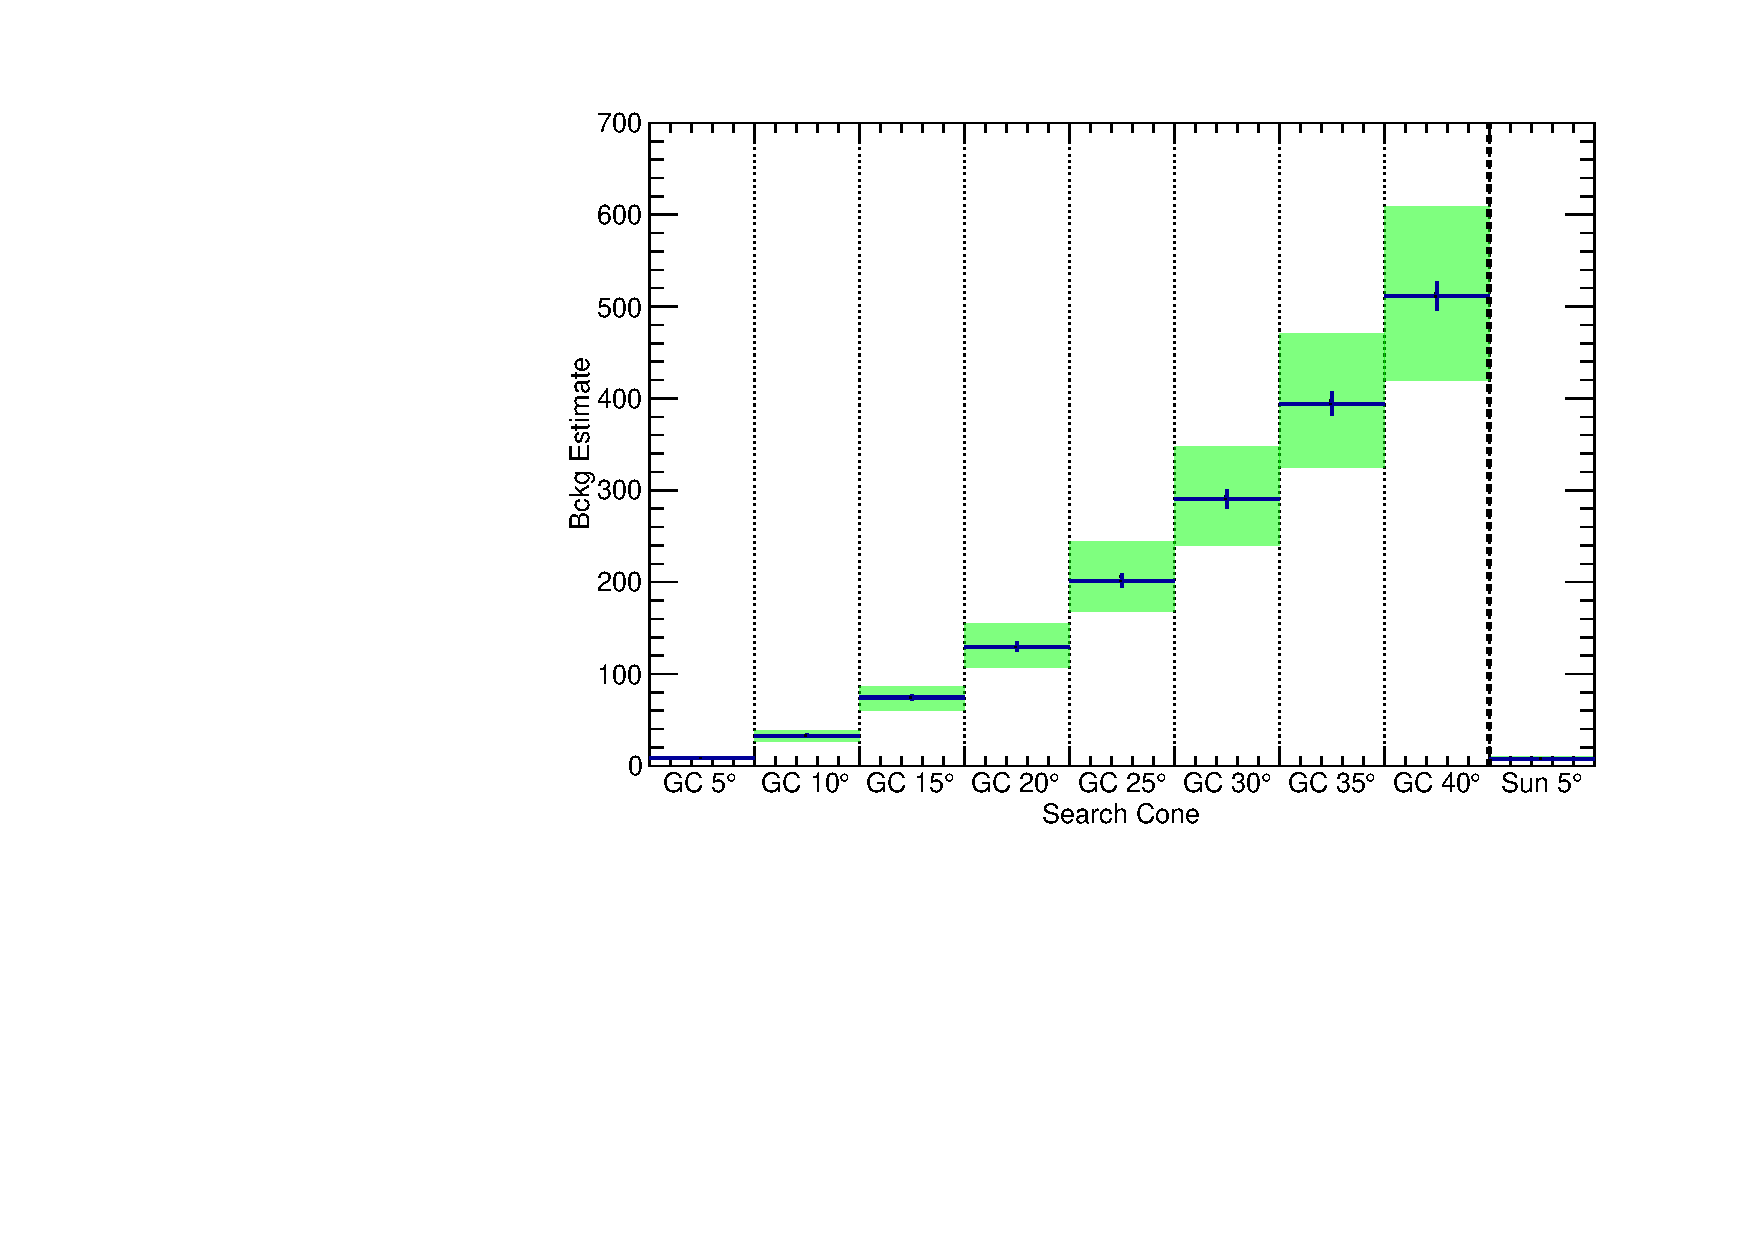
\includegraphics[width=0.45\textwidth]{figures/bckg_comparison_lowe.pdf}
	}
	\subfigure[Mid Energy]{
 	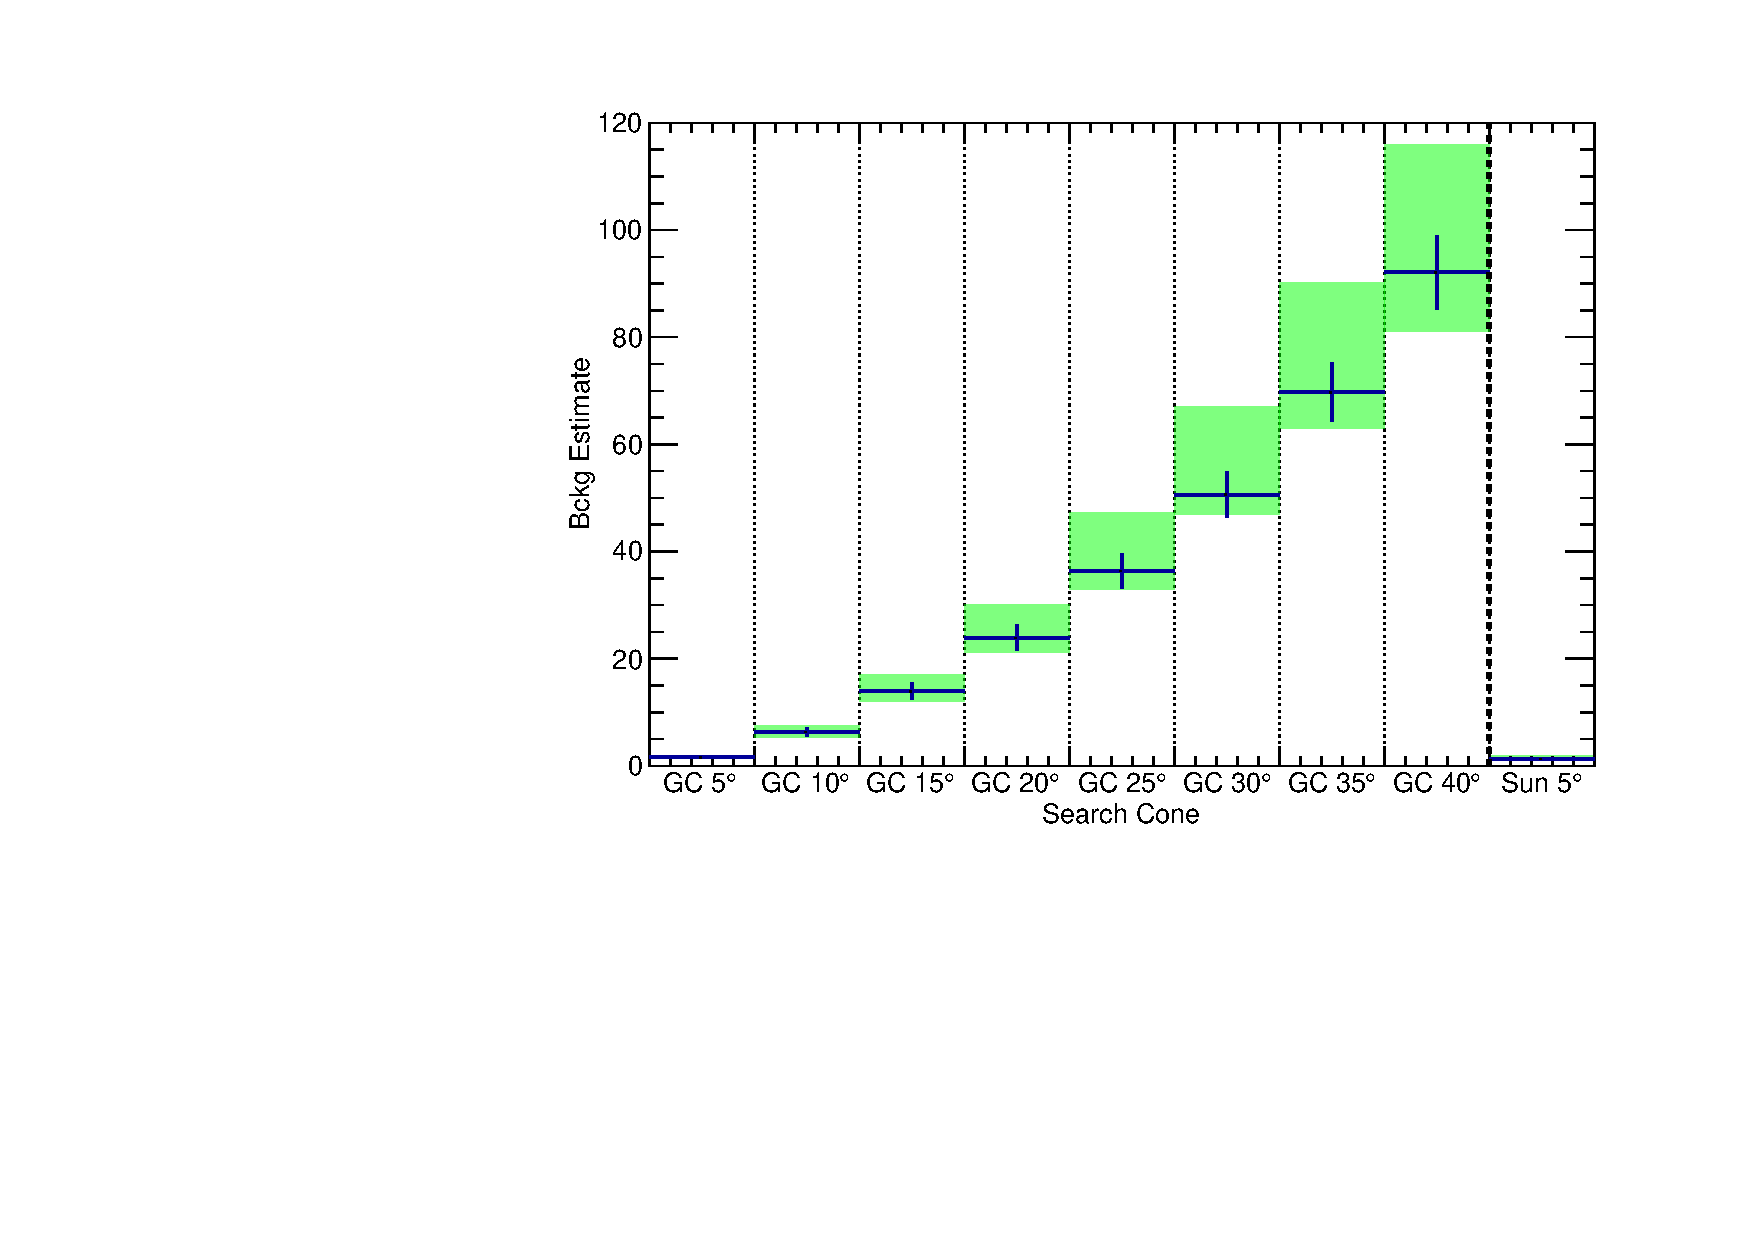
\includegraphics[width=0.45\textwidth]{figures/bckg_comparison_mide.pdf}
	}
	\caption{Comparison of AFS background estimates to MC background estimates for Low Energy and Mid Energy samples.  The two background estimation techniques agree to within systematic uncertainties, and the AFS technique has much smaller systematic uncertainties.}
	\label{fig:bckg_comparison}

\end{figure}



